\chapter{Introduction}
\label{ch:introduction}

\section{Preface}

\co{Different phases of matter exist and are determined by the way the atoms are organized.}
Even though all matter consists of atoms, it can appear in various forms and have various properties.
Familiar examples include solids, gases, and liquids; however, more exotic forms exists, such as gases, superfluids, magnets, plasmas, and Bose–Einstein condensates.
These different forms of matter are called phases or states of matter.
The various properties of materials arise from the different ``phases'' (ways atoms structure itself in a material).

\co{Symmetry-breaking theory explains how to understand the different phases of matter.}
Symmetry-breaking theory provides a way to understand many of the different phases.
It explains that these different phases correspond to different symmetries in the way the atoms are structured.
Whenever the order of a material changes (called a phase transition), the symmetry of the organization of the atoms changes.
For example, in a liquid the atoms are distributed randomly, and it remains a liquid upon moving the atoms by an arbitrary distance: it has a continuous translation symmetry.
When a liquid undergoes a phase transition and turns into a crystal (e.g.~water to ice) the atoms organize into a lattice.
The crystal \textit{only} remains the same if we move the atoms by an exact integer number of the lattice constant (the distance between the smallest repeating pattern): it has a discrete translation symmetry.
This phase transition is an example of symmetry breaking because it reduces the continuous translation symmetry of the liquid to the discrete symmetry of the crystal.
Another examples is ferromagnets, where the spins of electrons are randomly oriented above a certain critical temperature $T_c$: having a continuous rotational symmetry; while for $T<T_c$ the spin align: resulting in a discrete rotational symmetry.

\co{Symmetry-breaking theory works well but not for topologically ordered matter.}
This symmetry-breaking theory introduced by Lev Landau in 1937 has been a very successful theory \cite{Landau1937}.  % XXX: Do not say "has been a very successful theory"
It was long believed that the symmetry breaking theory explains all phases in materials and all (continuous) phase transitions.
In 1987, in an attempt to describe high $T_c$ superconductors, the chiral spin state was introduced \cite{Kalmeyer1987}.
However, it was soon realized that the symmetry breaking description was not sufficient to explain its phase.
A new kind of phase called a ``topological phase'' was introduced \cite{Wen1989,XiaoGang1990}.
It is a zero-temperature phase of matter (i.e.~quantum matter) that is described by a robust ground state degeneracy and has quantized non-Abelian geometric phases of degenerate ground states, we disscus what this means in Sec.~\ref{sec:non-abelian}.

\co{The QHE is an example that can be described using of the theory of topological order.}
The quantum Hall effect is an example of a state that cannot be described by its symmetries alone; instead, it can be characterized by a distinct topology (see Fig.~\ref{fig:knots}).
Its signature, shown in Fig.~\ref{fig:qhe}, is robust does not depend on the specific geometry and does not vanish upon smooth changes in material parameters.
This signature manifests in an exact quantization of the Hall conductance of an integer number of $e^2/h$, where $e$ is the elementary charge and $h$ is the Planck constant, both fundamental constants in nature.
Because of its robustness---it is insensitive to specific experimental settings and purity of the material used---the quantum Hall effect is used to determine the standard for electrical resistance.
The effect appears upon applying a large perpendicular magnetic field $B_\perp$ to two-dimensional electron gas at low temperature.
This opens a gap between the energy bands and localizes the electrons in the bulk.
Classically, we can visualize what happens as electrons localizing in small cyclotron orbits; this leaves the electrons near the edges of the material to bounce along the edges.
These states along the egdes are responsible for the conduction and are called ``edge states.''

\begin{figure}[!htb]
\centering
% \includegraphics{chapter_introduction/figures/knots.pdf}
\caption{
Topology in mathematics concerns itself with the properties of an object that are preserved under continuous deformations.
For example, an unknot (left) cannot be continuously transformed into a trefoil knot (right) without cutting it; this means that they are not topologically equivalent.
In condensed matter physics that object that is studied is the Hamiltonian.
Whenever the Hamiltonian can be continuously transformed into another Hamiltonian, they are topologically equivalent.
Unlike a knot that can be visualized in space, the topology of the quantum Hall state manifests itself in momentum space.
\label{fig:knots}}
\end{figure}

\begin{figure}[!htb]
\centering
% 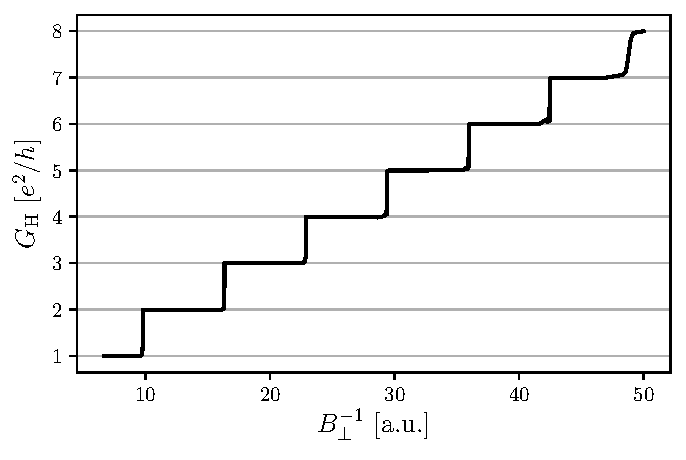
\includegraphics{chapter_introduction/figures/qhe.pdf}
\caption{
The integer quantum Hall effect.
The Hall resistance $R_H$ (reciprocal of the Hall conductance $G_H$) of a two-dimensional electron gas as a function of the perpendicular magnetic field $B_\perp$ at low-temperature.
It displays a stairlike quantized sequence of Hall conductances equal to $ne^2/h$, where $n$ is an integer characterizing each plateau.
\label{fig:qhe}}
\end{figure}

\co{More topological states have been realized, one example is TIs.}
The field of topology in condensed matter has substantially grown over the past decades.
Recently, in 2016, the Nobel prize was awarded to Thouless, Haldane, and Kosterlitz for the theoretical findings of topological states.
One of these new states are ``topological insulators,'' which also exhibit edge or surface states and have similarities to the quantum Hall effect, but do not require extreme conditions such as the large magnetic field.
Here, the effect of the magnetic field is replaced by spin-orbit coupling.
This is a coupling between the electron's momentum and spin, effectively causing a momentum dependent magnetic field for electrons that move through a crystal lattice.
The spin-orbit coupling effect is discussed in more detail in Sec.~\ref{sec:spin-orbit}.
Due to the absence of a magnetic field (which breaks time-reversal symmetry in the quantum Hall effect) the edge states always come in counter-propagating pairs, shown in see Fig.~\ref{fig:}.

\begin{figure}[!htb]
\centering
% \includegraphics{chapter_introduction/figures/qhe_vs_ti.pdf}
\caption{
Comparison of an insulator, quantum Hall effect, and a topological insulator.
% Rip Fig. 2 and 5 from 10.1103/RevModPhys.82.3045
\label{fig:qhe}}
\end{figure}

\co{Topological states might be used to build a topological quantum computer.}
In addition to the exciting new physical insights into topological materials, topological states might be used to design novel new quantum devices.
One of the most exciting applications is to use these states to build a topological quantum computer by exploiting their non-Abelian properties.
It is predicted that a quantum computer is much faster than a classical computer in performing certain tasks, such as the simulation of quantum systems \ref{Feynman1982} and prime factorization \cite{Shor1994}.
The fundamental building block of the quantum computer is the qubit (or quantum bits), the quantum equivalent of the classical transistor.
Because these qubits store quantum information, they are extremely fragile, and even a small interaction with its environment can destroy its state and result in computational errors.
Physicists experiment with different approaches to create a qubit; for example, there are proposals (and some realizations of) qubits based on quantum optics, ultracold atoms, spin-based systems, and superconducting systems.  % XXX: add refs
In general, one of the most significant problems is to limit and correct the computational errors, and therefore a large fraction of the research is focussed on error-correction \cite{Lidar2013}.
Here, the advantage of using topological states becomes apparent because the topological qubit naturally protects the its state against small perturbations in the environment \cite{Nayak2008}.

\co{Majoranas can be used to create this topological quantum computer.}
The simplest non-Abelian exitation is the zero-energy Majorana bound state (MBS), which were first proposed to exist as quasiparticle excitations of the $\nu = 5/2$ quantum Hall effect \cite{Read2000,Moore1991}, which requires a high material purity and very low temperatures.
Other early proposals \cite{Gurarie2005,Sarma2006,Tewari2007} rely on rare and exotic $p$-wave superconductors and are extremely challenging to realize
experimentally.
In 2008, Fu and Kane suggested a new approach to create MBSs by using a hybrid structure of an ordinary $s$-wave superconductor coupled to a topological insulator to create a state that resembles a spinless $p$-wave superconductor \cite{Fu2008}.
Inspired by this hybrid approach, in 2010, two works \cite{Lutchyn2010,Oreg2010} suggested using a simpler one-dimensional nanowire system coupled to a $s$-wave superconductor.
This simple model combines spin-orbit coupling, superconductivity, electrostatic tunability, and an applied magnetic field.
When tuned into the right parameter regime, this system hosts MBSs at the edges of the nanowire.
Since its introduction, many experiments have detected signatures of MBSs \cite{Mourik2012,Das2012,Deng2012,Deng2016,Deng2016a,Chen2017}; however, none have demonstrated the presence of MBSs with absolute certainty by showing its non-Abelian statistics.
Because of the simplicity of the model, it can be solved analytically; however, it neglects many physical phenomena that are crucial for understanding the properties of the MBSs.

\co{In this thesis we study the hybrid Majorana model.}
In this thesis, we study extensions to this model and go beyond the regime that can be studied analytically.
The next sections introduce superconductivity and the topological protection of Majoranas (Sec.~\ref{sec:?}), non-Abelian statistics (Sec.~\ref{sec:?}), the minimal hybrid Majorana model (Sec.~\ref{sec:?}), and finally, some extensions to this model (Sec.~\ref{sec:?}).
At that point, it should be evident that solving this problem requires numerical methods, which is the topic of Sec.~\ref{sec:?}.

\section{Structure of this thesis}

Here, we give a brief overview of the topics explored in the following chapters.
\vspace{1mm}

\subsection{Chapter~\ref{ch:introduction}: Introduction}
Abstract here for introduction
\vspace{1mm}

\subsection{Chapter~\ref{ch:adaptive}: Title here for adaptive}
Abstract here for adaptive
\vspace{1mm}

\subsection{Chapter~\ref{ch:orbitalfield}: Orbital effect of magnetic field on the Majorana phase diagram}
Studies of Majorana bound states in semiconducting nanowires frequently neglect the orbital effect of a magnetic field.
Systematically studying its role leads us to several conclusions for designing Majoranas in this system.
Specifically, we show that for experimentally relevant parameter values the orbital effect of a magnetic field has a stronger impact on the dispersion relation than the Zeeman effect.
While Majoranas do not require the presence of only one dispersion subband, we observe that the size of the Majoranas becomes unpractically large, and the band gap unpractically small, when more than one subband is filled.
Since the orbital effect of a magnetic field breaks several symmetries of the Hamiltonian, it leads to the appearance of large regions in parameter space with no band gap whenever the magnetic field is not aligned with the wire axis.
The reflection symmetry of the Hamiltonian with respect to the plane perpendicular to the wire axis guarantees that the wire stays gapped in the topologically nontrivial region as long as the field is aligned with the wire.
\vspace{1mm}

\subsection{Chapter~\ref{ch:supercurrent}: Supercurrent Interference in Few-Mode Nanowire Josephson Junctions}
Junctions created by coupling two superconductors via a semiconductor nanowire in the presence of high magnetic fields are the basis for the potential detection, fusion and braiding of Majorana bound states.
We study NbTiN/InSb nanowire/NbTiN Josephson junctions and find that the dependence of the critical current on the magnetic field exhibits gate-tunable nodes.
This is in contrast with a well-known Fraunhofer effect, under which critical current nodes form a regular pattern with a period fixed by the junction area.
Based on a realistic numerical model we conclude that the Zeeman effect induced by the magnetic field and the spin-orbit interaction in the nanowire are insufficient to explain the observed evolution of the Josephson effect.
We find the interference between the few occupied one-dimensional modes in the nanowire to be the dominant mechanism responsible for the critical current behavior.
We also report a strong  suppression of critical currents at finite magnetic fields that should be taken into account when designing circuits based on Majorana bound states.
\vspace{1mm}

\subsection{Chapter~\ref{ch:spinorbit}: Spin-Orbit Protection of Induced Superconductivity in Majorana Nanowires}
Spin-orbit interaction (SOI) plays a key role in creating Majorana zero modes in semiconductor nanowires proximity coupled to a superconductor.
We track the evolution of the induced superconducting gap in InSb nanowires coupled to a NbTiN superconductor in a large range of magnetic field strengths and orientations.
Based on realistic simulations of our devices, we reveal SOI with a strength of 0.15--0.35 eV\AA.
Our approach identifies the direction of the spin-orbit field, which is strongly affected by the superconductor geometry and electrostatic gates.
\vspace{1mm}

\subsection{Chapter~\ref{ch:zigzag}: Title here for zigzag}
Abstract here for zigzag
\vspace{1mm}

\subsection{Chapter~\ref{ch:shortjunction}: Robustness of Majorana bound states in the short-junction limit}
We study the effects of strong coupling between a superconductor and a semiconductor nanowire on the creation of the Majorana bound states, when the quasiparticle dwell time in the normal part of the nanowire is much shorter than the inverse superconducting gap.
This ``short-junction'' limit is relevant for the recent experiments using the epitaxially grown aluminum characterized by a transparent interface with the semiconductor and a small superconducting gap.
We find that the small superconducting gap does not have a strong detrimental effect on the Majorana properties.
Specifically, both the critical magnetic field required for creating a topological phase and the size of the Majorana bound states are independent of the superconducting gap.
The critical magnetic field scales with the wire cross section, while the relative importance of the orbital and Zeeman effects of the magnetic field is controlled by the material parameters only: $g$ factor, effective electron mass, and the semiconductor-superconductor interface transparency.

\subsection{Chapter~\ref{ch:weakantilocalization}: Title here for weakantilocalization}
Abstract here for weakantilocalization
\vspace{1mm}




\references{dissertation}
